%課題研究レジュメテンプレート ver. 1.2

\documentclass[uplatex]{jsarticle}
\usepackage[top=20mm,bottom=20mm,left=20mm,right=20mm]{geometry}
\usepackage[T1]{fontenc}
\usepackage{txfonts}
\usepackage{wrapfig}
\usepackage[expert,deluxe]{otf}
\usepackage[dvipdfmx,hiresbb]{graphicx}
\usepackage[dvipdfmx]{hyperref}
\usepackage{pxjahyper}
\usepackage{secdot}

\makeatletter
  \renewcommand{\section}{%
    \if@slide\clearpage\fi
    \@startsection{section}{1}{\z@}%
    {\Cvs \@plus.5\Cdp \@minus.2\Cdp}% 前アキ
    {.5\Cvs \@plus.3\Cdp}% 後アキ
    %{\normalfont\Large\headfont\raggedright}}
    {\normalfont\raggedright}}

  \renewcommand{\subsection}{\@startsection{subsection}{2}{\z@}%
    {\Cvs \@plus.5\Cdp \@minus.2\Cdp}% 前アキ
    {.5\Cvs \@plus.3\Cdp}% 後アキ
    %{\normalfont\large\headfont}}
    {\normalfont}}

  \renewcommand{\subsubsection}{\@startsection{subsubsection}{3}{\z@}%
    {\Cvs \@plus.5\Cdp \@minus.2\Cdp}%
    {\z@}%
    %{\normalfont\normalsize\headfont}}
    {\normalfont}}
\makeatother
%ここから上を編集する必要はない.





\title{\vspace{-14mm}研究タイトル}
\author{PMコース 矢吹研究室 1234567 氏名}
\date{}%日付を入れる必要はない.
\pagestyle{empty}%ページ番号は振らない.
\begin{document}
\maketitle



課題研究概要を2ページで書くこと.

提出前に\url{https://github.com/yabukilab/main/wiki/文章チェックリスト}を確認せよ.

\section{研究の背景}

\section{研究の目的}

\section{プロジェクトマネジメントとの関連}

\section{研究の方法}

%\begin{wrapfigure}[行数]{r}{幅}%行数はオプションだが,調整しないとうまくいかない.
\begin{wrapfigure}[13]{r}{5cm}
\vspace*{-\intextsep}
%\includegraphics[width=図の幅,clip]{ファイル名}\label{参照用ラベル}
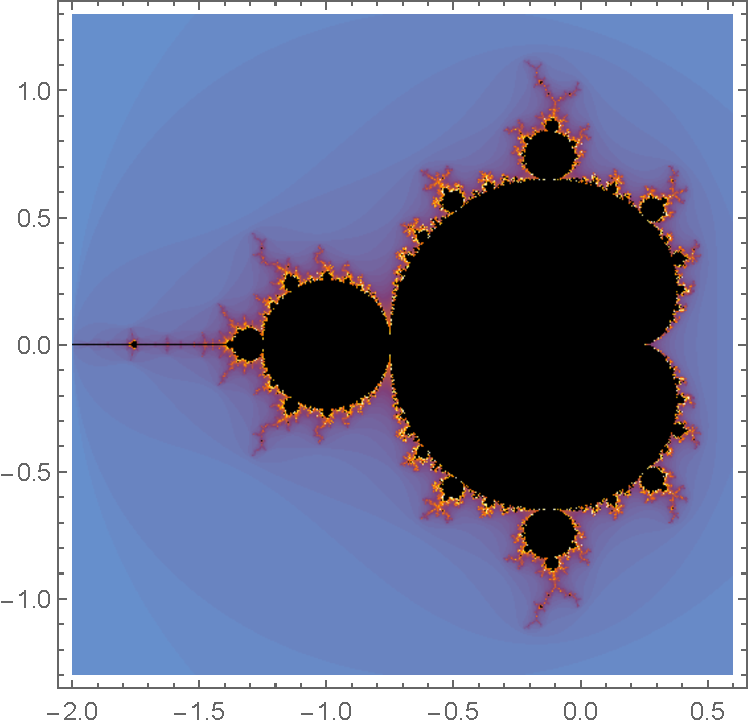
\includegraphics[width=5cm,clip]{figure.pdf}
\caption{図は\texttt{wrapfigure}環境を使って右側に寄せること.}\label{サンプル図}
\end{wrapfigure}

吾輩は猫である。名前はまだ無い。

どこで生れたかとんと見当がつかぬ。何でも薄暗いじめじめした所でニャーニャー泣いていた事だけは記憶している。吾輩はここで始めて人間というものを見た。しかもあとで聞くとそれは書生という人間中で一番獰悪な種族であったそうだ。この書生というのは時々我々を捕えて煮て食うという話である。しかしその当時は何という考もなかったから別段恐しいとも思わなかった。ただ彼の掌に載せられてスーと持ち上げられた時何だかフワフワした感じがあったばかりである。掌の上で少し落ちついて書生の顔を見たのがいわゆる人間というものの見始であろう。この時妙なものだと思った感じが今でも残っている。第一毛をもって装飾されべきはずの顔がつるつるしてまるで薬缶だ。その後猫にもだいぶ逢ったがこんな片輪には一度も出会わした事がない。のみならず顔の真中があまりに突起している。そうしてその穴の中から時々ぷうぷうと煙を吹く。どうも咽せぽくて実に弱った。これが人間の飲む煙草というものである事はようやくこの頃知った。

%\begin{wraptable}[行数]{r}{幅}%行数はオプションだが,調整しないとうまくいかない.
\begin{wraptable}[8]{r}{4cm}
\vspace*{-\intextsep}
\caption{図は\texttt{wraptable}環境を使って右側に寄せること.}\label{サンプル表}
\begin{tabular}{cc}
\hline
文字 & コードポイント \\
\hline
\UTF{005C} & U+005C\\
\UTF{00A5} & U+00A5\\
\hline
\end{tabular}
\end{wraptable}

この書生の掌の裏でしばらくはよい心持に坐っておったが、しばらくすると非常な速力で運転し始めた。書生が動くのか自分だけが動くのか分らないが無暗に眼が廻る。胸が悪くなる。到底助からないと思っていると、どさりと音がして眼から火が出た。それまでは記憶しているがあとは何の事やらいくら考え出そうとしても分らない。

ふと気が付いて見ると書生はいない。たくさんおった兄弟が一疋も見えぬ。肝心の母親さえ姿を隠してしまった。その上今までの所とは違って無暗に明るい。眼を明いていられぬくらいだ。はてな何でも容子がおかしいと、のそのそ這い出して見ると非常に痛い。吾輩は藁の上から急に笹原の中へ棄てられたのである。

\section{現在の進捗状況}

\section{今後の計画}

文献の種類には,雑誌論文\cite{yabuki2011}や会議録論文\cite{数式処理システムの性能評価},卒業論文\cite{kubo2014},書籍\cite{okumura2017},ウェブサイト\cite{文章チェックリスト}などがある.文献の種類によって必要な項目が異なるため,文献\cite{参考文献リストの書き方}を見て確認すること.(注意:文献番号は句読点の前に書く.)

\bibliographystyle{junsrt}
\bibliography{biblio}%「biblio.bib」というファイルが必要.

\end{document}
